\documentclass[12pt]{article}
 
\usepackage[margin=1in]{geometry} 
\usepackage{amsmath,amsthm,amssymb,enumitem, wasysym}
\usepackage{slashed}
\usepackage{tikz}
\usepackage{hyperref, parskip}
\hypersetup{
    colorlinks=true,
    linkcolor=magenta,
    filecolor=magenta,      
    urlcolor=blue,
}
\newcommand{\N}{\mathbb{N}}
\newcommand{\Z}{\mathbb{Z}}
\DeclareMathOperator{\Q}{\mathbb{Q}}
\DeclareMathOperator{\R}{\mathbb{R}}
\usepackage[T1]{fontenc}
 
\newenvironment{lemmaNoNum}[2][Lemma 1:]{\begin{trivlist}
\item[\hskip \labelsep {\bfseries #1}]}{\end{trivlist}}

\begin{document}
We've been running our own implementation of BOLA-BASIC alongside BBA and other ABR algorithms on Puffer since 6/9. The results are
\href{https://puffer.stanford.edu/results/}{here}, and the code is \href{https://github.com/StanfordSNR/puffer/blob/master/src/abr/bola_basic.cc}{here} and \href{https://github.com/StanfordSNR/puffer/blob/master/src/abr/bola_basic.hh}{here}. 

Here is a summary of BOLA's performance versus BBA's thus far:\\
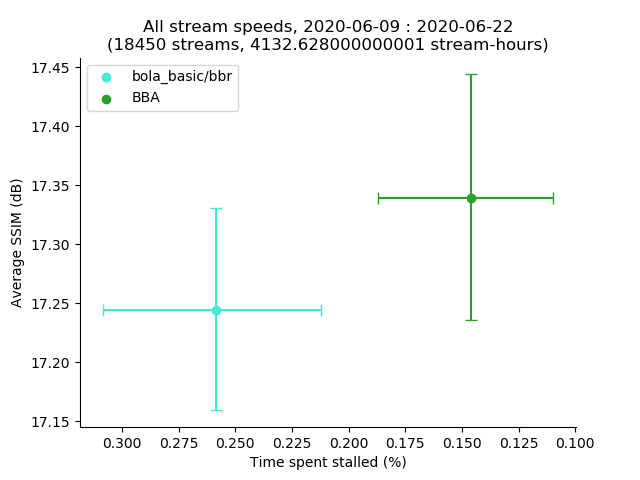
\includegraphics[width=0.7\textwidth]{duration_all_plot.png}\\
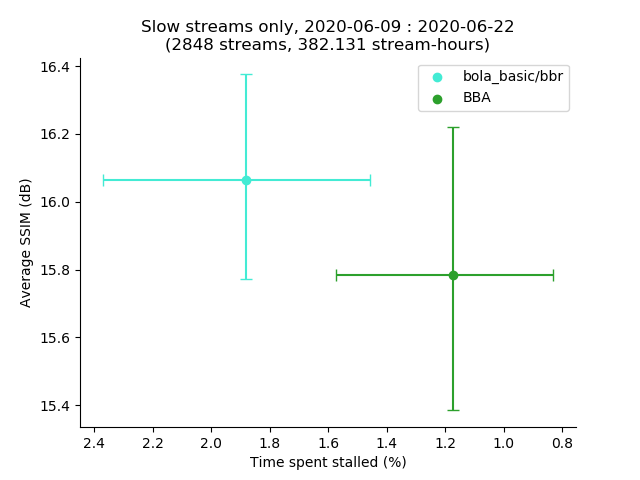
\includegraphics[width=0.7\textwidth]{duration_slow_plot.png}

\textbf{Figure A:} Performance of BOLA vs BBA on Puffer. Better performance is toward the top right.
\newpage
We want to represent BOLA fairly on Puffer, so please let us know if there's anything we should consider changing in our current implementation (described below, in perhaps too much detail). In particular, we have two main questions -- we'd much appreciate any thoughts: \\

\begin{enumerate}
    \item 
We use SSIM in decibels (SSIMdB) as the utility function. We suspect that the relationship between SSIMdB and chunk size introduces some surprising behavior, described in Figure E below. So, we were curious if you had any thoughts on using a utility function involving metrics not strictly linear in size (see \hyperref[sec:Utility]{\textbf{Utility (SSIMdB)}} below).
\item
Because we deployed BOLA-BASIC on Puffer before \href {https://arxiv.org/pdf/1601.06748.pdf}{v3} of the paper was available, we had to extrapolate a bit from v2 in order to calculate $V$ and $\gamma$ based on our min/max buffer targets. Fortunately, we ended up solving exactly equations (13) and (14) in the \textit{BOLA Parameters} section of v3. Our solution to these two equations (in code \href{https://github.com/StanfordSNR/puffer/blob/master/src/abr/bola_basic.hh}{here}) is also almost equivalent to the paper's, except for a negation on $\alpha$. Our solution is attached -- we took a slightly different path with the algebra than the paper, so there's a bit of rearrangement at the end. We also used our final expressions for $V$ and $\gamma$ along with the buffer levels in Figures 1 and 2 (which we calculated as min 12.0573099287 sec, max 22.0337358802 sec) to recover the parameter values stated in the paper, i.e. $V = 0.93$ and $\gamma p = 5$. Without the negation on $\alpha$, we instead get $V = 1.49862824818$ and $\gamma p = 2.0034712277$. But, we're certainly happy to be corrected!	 	
\end{enumerate} 

Following is more information about our BOLA-BASIC implementation on Puffer. 
 
\section*{Puffer background} 
There are a few differences between Puffer and many client-side DASH players: 
\begin{enumerate}
    \item 
All ABR algorithms are implemented on the server side in Puffer. Each streaming session (a "session" begins when the player loads, and is maintained across channel changes) uses a single WebSocket connection, rather than DASH HTTP request/response pairs. 
\item
Puffer exclusively serves live streams of indeterminate length. 
\item
On each of Puffer's channels, each 120-frame (2.002-second) chunk is encoded in ten formats using x264 in CRF mode. The size and SSIM of each of the ten formats is available only at runtime. (SSIM is a video quality metric based on structural similarity; it is unusual to have per-format SSIM information at runtime).

\end{enumerate} 
\newpage
\section*{Utility (SSIMdB)}
\label{sec:Utility}
For BOLA's utility function, we convert the raw SSIM value (between 0 and 1) to decibels, using the function \href{https://github.com/StanfordSNR/puffer/blob/master/src/abr/abr_algo.cc}{here} (a log10 with some arithmetic). The resulting value is most commonly between 10 and 18 dB, although the theoretical range is 0 to 60 dB. \\
 
SSIMdB is believed to be linear with perceived quality, nondecreasing with format size, and \textit{generally} concave with format size. However, we have found instances where concavity doesn't strictly hold, e.g. for certain timestamps in a 10-minute CBS clip. One such timestamp is shown in Figure B below. Notice the third-smallest chunk would be chosen at startup here.\\

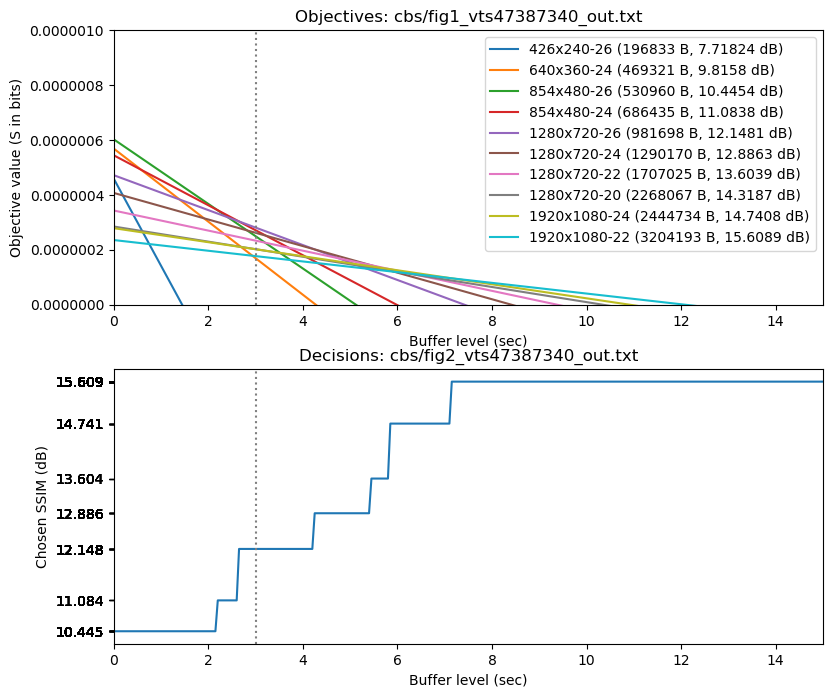
\includegraphics[width=0.9\textwidth]{single_vts47387340.png} \\
\textbf{Figure B:} Nonconcavity of SSIMdB with respect to size.
 
We use the SSIMdB value directly, without normalization. We do notice that normalizing (such that the smallest utility is zero) keeps $\gamma$ positive, but in our case the smallest utility could take any value. For instance, it's possible to have a format with zero SSIMdB. So, we're wondering whether normalization makes sense when using a utility function like SSIMdB for BOLA -- namely, a function that can vary independently of size.

\section*{Parameter Calculation}
We define the minimum buffer level (3 seconds, as in our BBA implementation) as the level at which the objectives for the smallest and second-smallest formats intersect. We define the maximum buffer level (15 seconds) as the level above which no chunk is sent. This maximum is enforced by Puffer's media server regardless of the ABR algorithm assigned to a session.
 
To calculate $V$ and $\gamma$, we solve (13) and (14) from v3 of the paper. As mentioned above, our solution negates $\alpha$ relative to the paper (algebra attached). 
 
We calculate the parameters statically, whereas the sizes and utilities of the ten format options are unknown until runtime. So, to produce the static size and SSIM "ladders" used to calculate the parameters, we average the encoded sizes and SSIMs for each format option across channels, over a week of 2019 Puffer data. 
 
The resulting values are $V = 0.672884$ and $\gamma p = -6.6447$ ($p$ is technically dynamic, but in practice is 2.002 sec). Note again that SSIMdB is not normalized, and $\gamma p$ is negative. (There is a note about the sign of $\gamma$ on the last page of the attached math). 
 
Figure C  below is the equivalent of Figures 1 and 2 in the BOLA paper (plotting SSIM rather than size for Fig 2), where the static ladders mentioned above are used as the "encoded formats" whose objectives are plotted. In other words, this is the figure we'd see if the ten encoded formats produced by x264 at some time slot exactly matched the average sizes/SSIMs from a week of 2019 data.  Note the static ladders can be read from the legend. \\
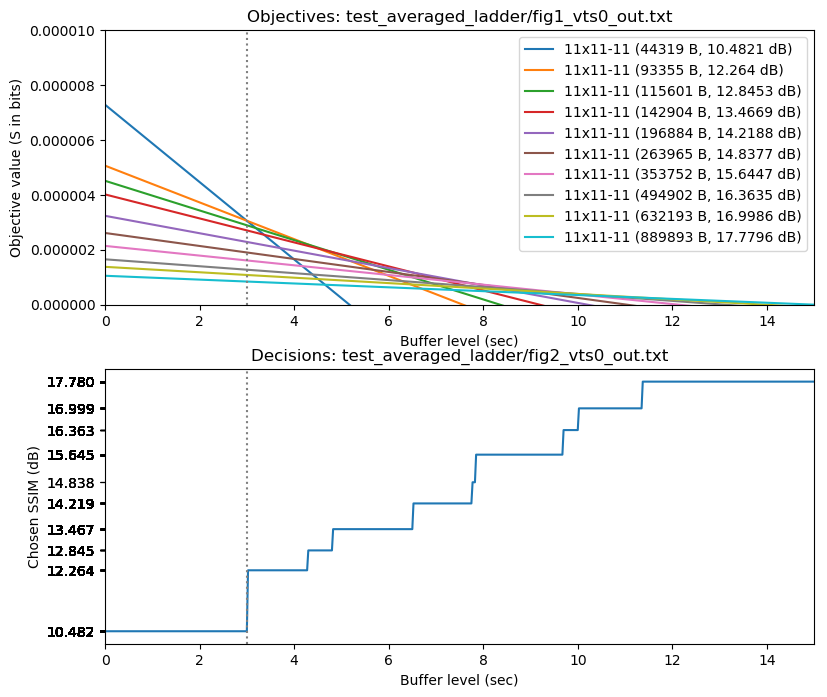
\includegraphics[width=0.9\textwidth]{test_averaged_ladder.png} \\
\textbf{Figure C:} Objectives and format decisions using static ladders. Minimum buffer is 3sec (grey dashed line), maximum buffer is 15 sec. 
 
We've also produced Figures 1 and 2 for each 120-frame chunk of a 10-minute CBS clip (300 chunks). The figures are \href {https://console.cloud.google.com/storage/browser/puffer-stanford-public/BOLA/cbs}{here}; the number in each figure's name is the presentation timestamp of the chunk, which starts at 0 and increments by 180180 for each 120-frame chunk. If extreme timestamps are of interest, timestamp 37117080 has the smallest minimum size (5029B, as compared to the average min of 44,319B), and timestamp 47387340 has the largest min size (196,833B). Timestamp 47387340 is also the nonconcave timestamp shown in Figure B.
 
Figure D below places all 300 timestamps in the Figures 2 (chosen utility) from the CBS clip onto a single plot, and plots the equivalent for size as well:\\
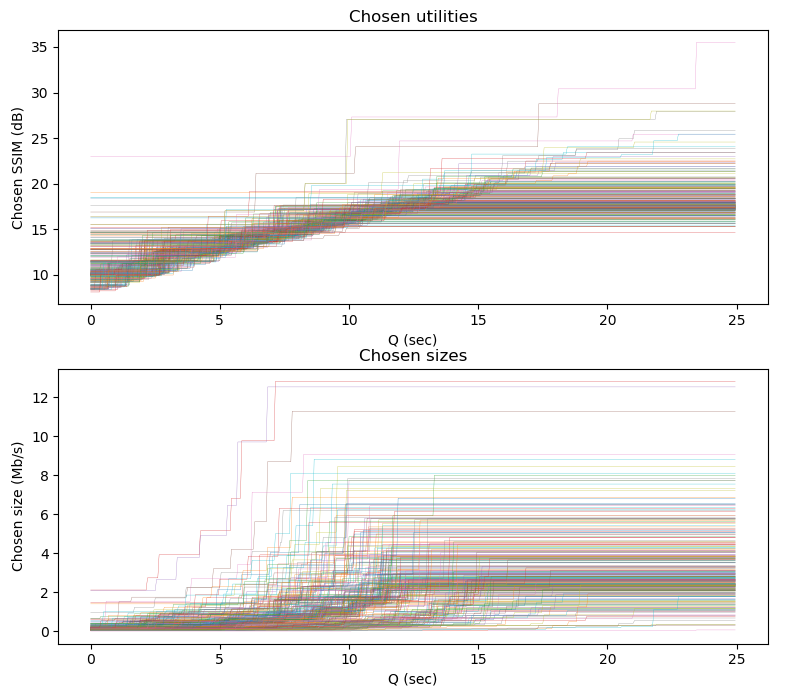
\includegraphics[width=0.9\textwidth]{shared_decisions_2.png} \\

\textbf{Figure D:} Utilities and sizes of chosen formats over a 10-minute clip. Each line on each subplot represents a single 120-frame chunk. The x-axis goes up to 25 sec, so the region past 15 sec (the maximum buffer size) is entirely hypothetical.
 
Finally, in Figure E, we show the SSIM increases required for BOLA to prefer a larger format, with the buffer fixed at empty.\\\\
\hspace*{-3cm}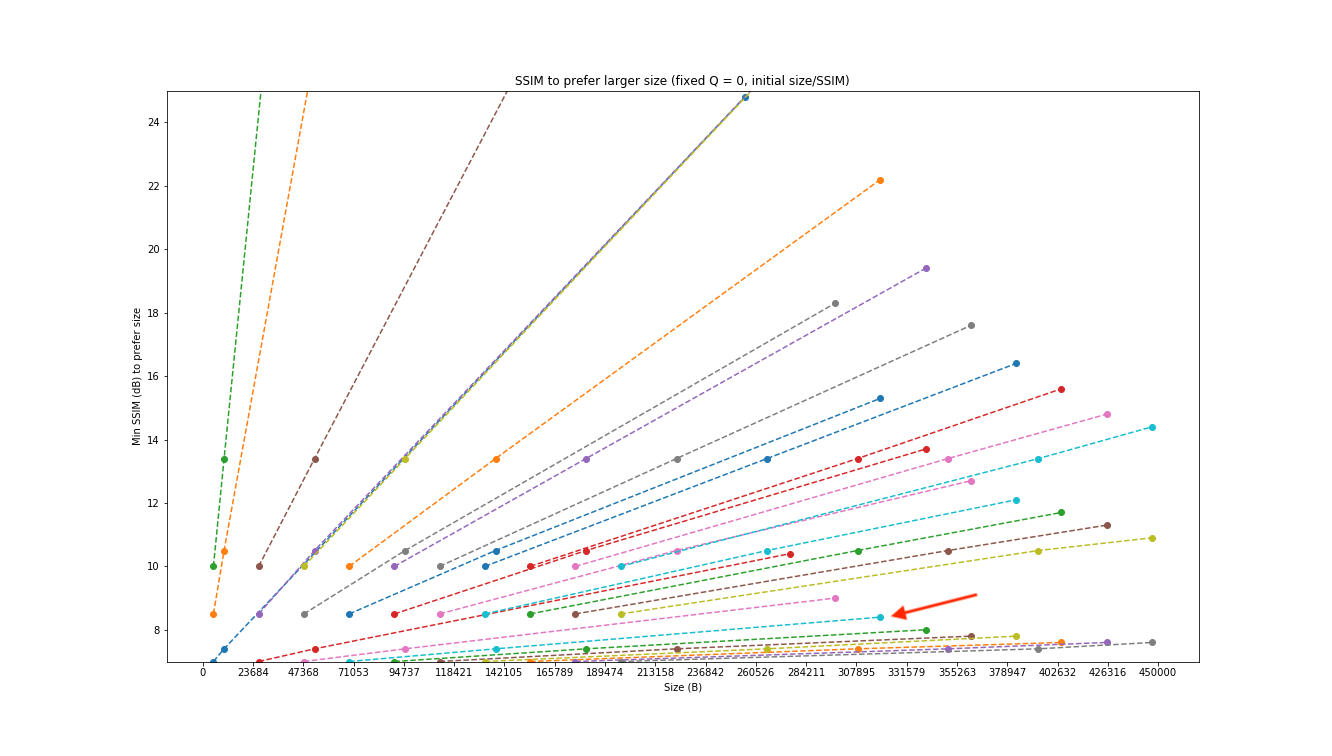
\includegraphics[width=1.3\textwidth]{ssim_to_prefer_sz.png} 
\textbf{Figure E:} SSIMdB increase required to prefer a larger format, as compared to a reference format of arbitrary size and SSIM. Each line represents one reference format. 
 
Each line in Figure E has three points (the y-axis is limited to 25, since the average maximum SSIMdB is 17.8 dB, so some points may be cut off). The first point on each line is a "reference format" with some arbitrary $size_0$ and $SSIM_0$. Another point is the smallest possible SSIMdB that a format of size $2 * size_0$ can have, such that BOLA will prefer it over the reference format despite its larger size. Similarly, a third point is the minimum-SSIMdB format with size 1 Mbps (250,250B) larger than $size_0$ that BOLA will prefer over the reference. (The order of the points depends on the relative values of $2 * size_0$ and 1Mbps $ + size_0$).
 
We were surprised that when two options are available with very different sizes, the much larger option may be selected due to a very slightly larger SSIMdB (especially keeping in mind that the buffer is empty here). For instance, in the cyan line identified by the red arrow in Fig. E, the reference format is 68,964 B with 7.0 SSIMdB. To get the next point on that line, we fix size at twice the reference (137,927B), and increase SSIMdB until the objective is higher than the reference. At this point, we plot the resulting SSIMdB against the doubled size (137,927B). The resulting SSIMdB is only 7.4, as compared to 7.0 in the reference. In other words, even with an empty buffer, we would prefer a format twice as large offering only a 0.4dB SSIM increase. (The third point on the cyan line is 319,214B, 8.4dB.)
\end{document}
